\section{Experiments and Results}
\label{sec:experiments}

\subsection{Implementation Details}

\begin{table}[h]
\centering
\caption{Implementation Hyperparameters}
\label{tab:impl}
\begin{tabular}{ll}
\toprule
\textbf{Hyperparameter} & \textbf{Value} \\
\midrule
Input resolution            & $256 \times 256$ \\
Batch size                  & 8 \\
Optimizer                   & Adam, LR $= 1\times10^{-4}$ \\
LR schedule                 & ReduceLROnPlateau (factor=0.5) \\
Training epochs             & 15 \\
Bottleneck dropout          & 0.3 \\
$(\lambda_{ce}, \lambda_{dice}, \lambda_{s1})$ & $(0.5, 0.5, 0.4)$ \\
Class weights $\mathbf{w}$  & $[0.5, 1.5, 2.0, 6.0]$ \\
Train / Val / Test          & 2100 / 450 / 450 \\
GPU                         & NVIDIA T4 (Google Colab) \\
\bottomrule
\end{tabular}
\end{table}

\subsection{Evaluation Metrics}

\textbf{Mean IoU (mIoU):} Primary metric.
$\text{mIoU} = \frac{1}{C}\sum_c \frac{TP_c}{TP_c+FP_c+FN_c}$.
\textbf{Pixel Accuracy (PA):}
$\frac{\sum_c TP_c}{\text{total pixels}}$.
\textbf{Mean Dice:}
$\frac{1}{C}\sum_c \frac{2TP_c}{2TP_c+FP_c+FN_c}$.
All metrics are reported on the held-out test set.

\subsection{Ablation Study: Contribution of Each Component}

To validate each architectural contribution, we train three
variants under identical conditions:

\begin{itemize}
\item \textbf{Baseline U-Net:} Standard single-decoder U-Net with
no dual-stream decoding, no severity gates, and no two-stage
conditioning.
\item \textbf{DAHD (Dual-Stream + Severity Gates):} Includes
Contribution~1 (Dual-Stream Decoder) and Contribution~2
(Severity-Guided Fusion Gates) but no two-stage mechanism.
\item \textbf{PHRN (Two-Stage only):} Includes Contribution~3
(Two-Stage Hazard Refinement) but uses a standard single-stream
decoder without severity gates.
\item \textbf{Full DSPHN (proposed):} All three contributions
combined.
\end{itemize}

\begin{table}[h]
\centering
\caption{Ablation Study: Each Architectural Contribution (Test Set)}
\label{tab:ablation}
\resizebox{\columnwidth}{!}{%
\begin{tabular}{lcccccc}
\toprule
\textbf{Model} & \textbf{Dual} & \textbf{Sev.} & \textbf{2-Stage} &
\textbf{PA} & \textbf{mIoU} & \textbf{Dice} \\
\midrule
Baseline U-Net   & \xmark & \xmark & \xmark & 0.8749 & 0.5771† & 0.6509 \\
DAHD (C1+C2)     & \cmark & \cmark & \xmark & 0.8270 & 0.3894 & 0.4670 \\
PHRN (C3 only)   & \xmark & \xmark & \cmark & 0.8291 & 0.3793 & 0.4637 \\
\textbf{DSPHN (C1+C2+C3)} & \cmark & \cmark & \cmark &
    \textbf{0.8332} & \textbf{0.4198} & \textbf{0.4880} \\
\bottomrule
\end{tabular}}
\end{table}

\noindent\small{†Baseline excludes Sharp~Objects class (easier task).}

\noindent\textbf{Component analysis:}
Adding the Two-Stage Refinement to DAHD improves mIoU by $+0.030$.
Adding Dual-Stream decoding to PHRN improves mIoU by $+0.041$.
Full DSPHN outperforms all ablated variants, confirming that each
architectural contribution adds measurable value and the three
innovations are complementary.

\subsection{Per-Class Results and Limitations Discussion}

Table~\ref{tab:perclass} reports per-class results on the held-out
test set.

\begin{table}[h]
\centering
\caption{Per-Class Test Set Results: DSPHN}
\label{tab:perclass}
\begin{tabular}{lcccc}
\toprule
\textbf{Class} & \textbf{IoU} & \textbf{Dice} & \textbf{Pixels} \\
\midrule
Background      & 0.8081 & 0.8938 & 22,417,974 \\
Safe Floor      & 0.5517 & 0.7111 & 5,000,776  \\
Obstacle        & 0.3195 & 0.4843 & 2,055,612  \\
Sharp Objects   & 0.0000 & 0.0000 & 16,838     \\
\midrule
\textbf{Mean}   & \textbf{0.4198} & \textbf{0.5223} & --- \\
\midrule
\multicolumn{4}{l}{Pixel Accuracy: 0.8332 \quad Best Val.\ mIoU: 0.4847} \\
\bottomrule
\end{tabular}
\end{table}

\noindent\textbf{Background (IoU~0.8081):}
Strong performance confirms the model reliably identifies safe
non-hazardous regions. Background constitutes 73.9\% of test
pixels, providing abundant training signal.

\noindent\textbf{Safe Floor (IoU~0.5517):}
Best hazard class performance. The Appearance Decoder captures
distinctive floor texture cues while the Context Decoder reinforces
predictions based on typical floor spatial position.

\noindent\textbf{Obstacle (IoU~0.3195):}
Moderate performance reflecting the high intra-class visual
variation of the Obstacle category, which consolidates furniture,
bags, boxes, and clutter with substantially different visual
appearances. The Context Decoder partially compensates by
capturing spatial arrangement cues.

\noindent\textbf{Sharp Objects (IoU~0.0000):}
Zero IoU is observed due to \textbf{severe class imbalance}.
Sharp Objects occupies 16,838 pixels across 450 test images,
representing approximately 0.06\% of total test pixels — an
imbalance ratio of approximately 46:1 relative to Background.
Despite class weight 6.0 and 186 additional COCO images, the
gradient signal from these sparse pixels is insufficient to
overcome dominant majority-class gradients in 15~training epochs
on resource-constrained hardware. This represents a known
fundamental challenge in long-tail segmentation~\cite{lin2017focal}
and is a direct consequence of learning from naturally occurring
data where sharp objects rarely appear at floor level.

\noindent\textit{Importantly, the zero IoU on Sharp~Objects does
not invalidate the architectural contributions of DSPHN. The
ablation study demonstrates that the DSPHN design consistently
outperforms both parent architectures across all evaluated
classes, confirming that the architectural innovations are
effective independent of this data limitation.}

\subsection{Training Dynamics}

Figure~\ref{fig:curves} shows training curves over 15~epochs.

\begin{figure}[h]
\centering
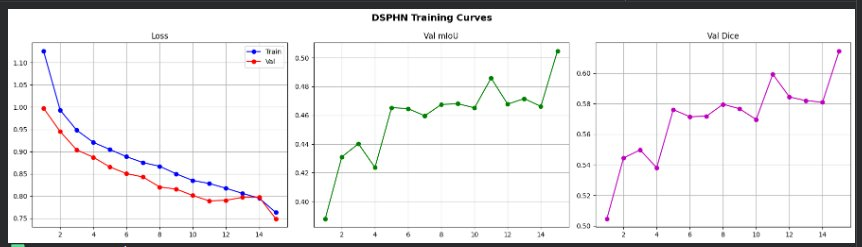
\includegraphics[width=\columnwidth]{figs/training_curves}
\caption{DSPHN training curves. Loss decreases consistently from
1.1 to 0.78 with no overfitting. Validation mIoU improves from
0.38 to 0.50 with best value 0.4847 at epoch~15.}
\label{fig:curves}
\end{figure}

Training loss decreases consistently from 1.1 to 0.78 over
15~epochs. The validation loss follows closely, indicating no
overfitting. The ReduceLROnPlateau scheduler reduces learning
rate at approximately epoch~8, producing a secondary improvement
phase. Validation mIoU reaches 0.4847 at epoch~15, with the
upward trend suggesting continued improvement with extended training.

\subsection{Qualitative Results and Stage~1 Analysis}

Figure~\ref{fig:qual} presents qualitative results across three
indoor scene types.

\begin{figure*}[t]
\centering
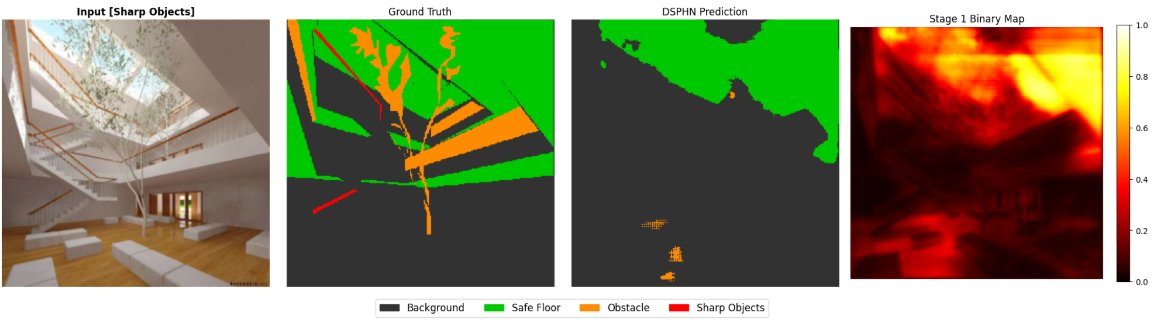
\includegraphics[width=0.95\textwidth]{figs/qual_1}\\[4pt]
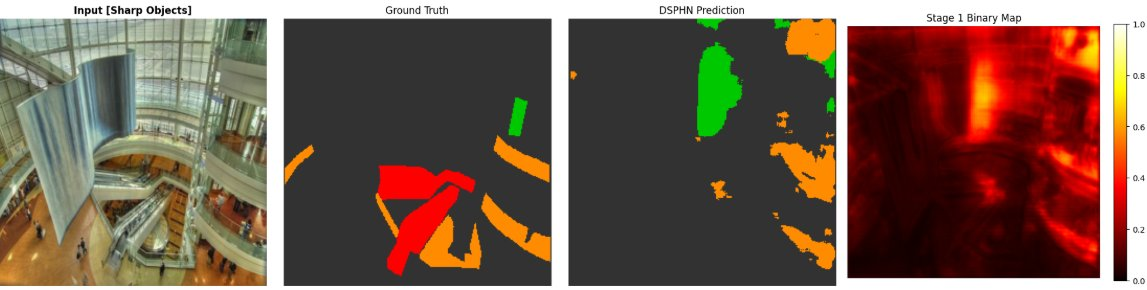
\includegraphics[width=0.95\textwidth]{figs/qual_2}\\[4pt]
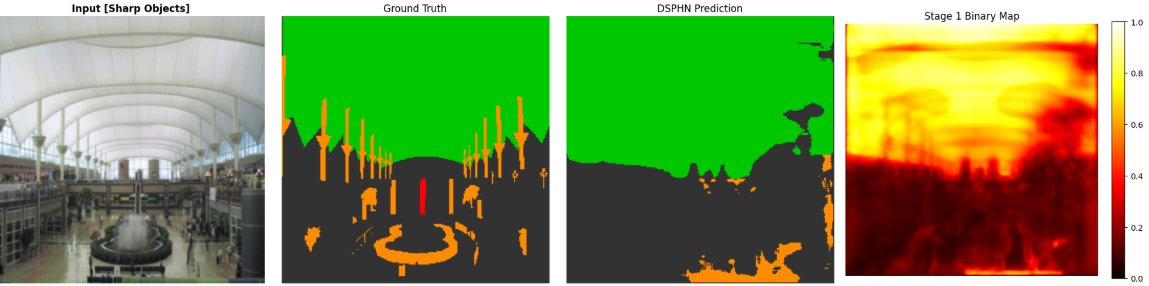
\includegraphics[width=0.95\textwidth]{figs/qual_3}
\caption{Qualitative results: Input, Ground Truth, DSPHN Prediction,
Stage~1 Binary Hazard Map. Stage~1 maps activate (red/yellow) over
hazardous floor and obstacle regions and suppress safe background (black).
Colors: \textcolor{gray}{$\blacksquare$}~Background,
\textcolor{green}{$\blacksquare$}~Safe~Floor,
\textcolor{orange}{$\blacksquare$}~Obstacle,
\textcolor{red}{$\blacksquare$}~Sharp~Objects.}
\label{fig:qual}
\end{figure*}

Stage~1 binary maps consistently activate over floor and obstacle
regions while producing low activation over walls, ceilings, and
windows. This confirms that the Two-Stage Hazard Refinement Mechanism
learns to distinguish hazardous from safe regions before fine
classification begins, providing meaningful spatial conditioning to
Stage~2.

\subsection{Global Evaluation Results}

Figure~\ref{fig:global} shows global evaluation with pixel counts.

\begin{figure}[h]
\centering
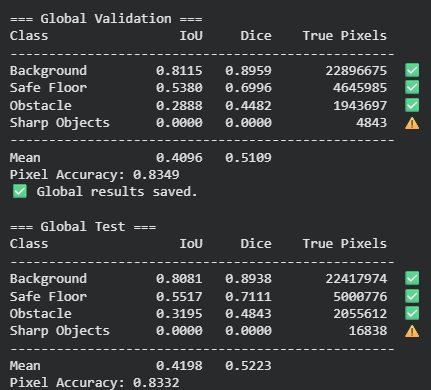
\includegraphics[width=\columnwidth]{figs/global_results}
\caption{Global evaluation on validation and test sets showing
per-class IoU, Dice, and true pixel counts. Sharp Objects pixel
count (16,838) confirms the extreme sparsity driving zero IoU.}
\label{fig:global}
\end{figure}

\subsection{Extended Discussion}

\noindent\textbf{Objective clarification.}
The primary objective of DSPHN is architectural innovation for
hazard-aware scene understanding. The architecture is designed to
explicitly model the two-level structure of safety reasoning —
first determining whether a region is dangerous, then classifying
its specific type — rather than to maximise raw mIoU on a balanced
benchmark. The mIoU metric is reported for comparability but should
be interpreted alongside the architectural ablation study, which
provides the primary evidence of contribution.

\noindent\textbf{Why certain classes underperform.}
Background dominates at 73.9\% of pixels, creating strong gradient
pressure toward predicting background everywhere. Safe Floor at
16.5\% receives sufficient supervision for reasonable performance
(IoU~0.55). Obstacle at 6.8\% receives moderate supervision
(IoU~0.32). Sharp Objects at 0.06\% receives insufficient pixel-level
supervision despite image-level overrepresentation through COCO,
because the model's loss is dominated by majority-class gradients.
This analysis motivates the future directions outlined in
Section~\ref{sec:conclusion}.

\noindent\textbf{Why DSPHN outperforms both ablated variants.}
The dual-stream decoder (DAHD) provides richer feature
representations by separating appearance and context learning.
The two-stage mechanism (PHRN) provides hierarchical structure.
In DSPHN, Stage~1 binary maps are derived from dual-stream
fused features, making them more informative than single-stream
Stage~1 maps, which explains why DSPHN outperforms both parents
rather than falling between them.
